%----------------------------------------------------------------------------------------
%	PACKAGES AND OTHER DOCUMENT CONFIGURATIONS
%----------------------------------------------------------------------------------------

\documentclass[9pt]{developercv}
\usepackage{graphicx}
\usepackage[export]{adjustbox}
%----------------------------------------------------------------------------------------

\begin{document}

%----------------------------------------------------------------------------------------
%	TITLE AND CONTACT INFORMATION
%----------------------------------------------------------------------------------------

\begin{minipage}[t]{0.3\textwidth}
	\vspace{-\baselineskip}
	\colorbox{black}{{\Huge\textcolor{white}{\textbf{\MakeUppercase{Ionut Daniel}}}}}
	
	\colorbox{black}{{\Huge\textcolor{white}{\textbf{\MakeUppercase{Fagadau}}}}}
	
	\vspace{6pt}
	
	{\Large 17 Gennaio 1999 \\ Dorohoi, Romania}
\end{minipage}
\begin{minipage}[t]{0.22\textwidth} 
	\vspace{-\baselineskip}
	
	\icon{MapMarker}{12}{Trecate, Novara}\\
	\icon{Phone}{12}{+39 3890989121}\\
\end{minipage}
\begin{minipage}[t]{0.3\textwidth}
\vspace{-\baselineskip}
\icon{At}{12}{danielfagadau@gmail.com}\\
	\icon{Linkedin}{12}{\href{https://www.linkedin.com/in/daniel-fagadau/}{daniel-fagadau}} \\	
\end{minipage}
\begin{minipage}[t]{0.2\textwidth}
\vspace{-\baselineskip}
\noindent
\centering
\vspace{-20mm}{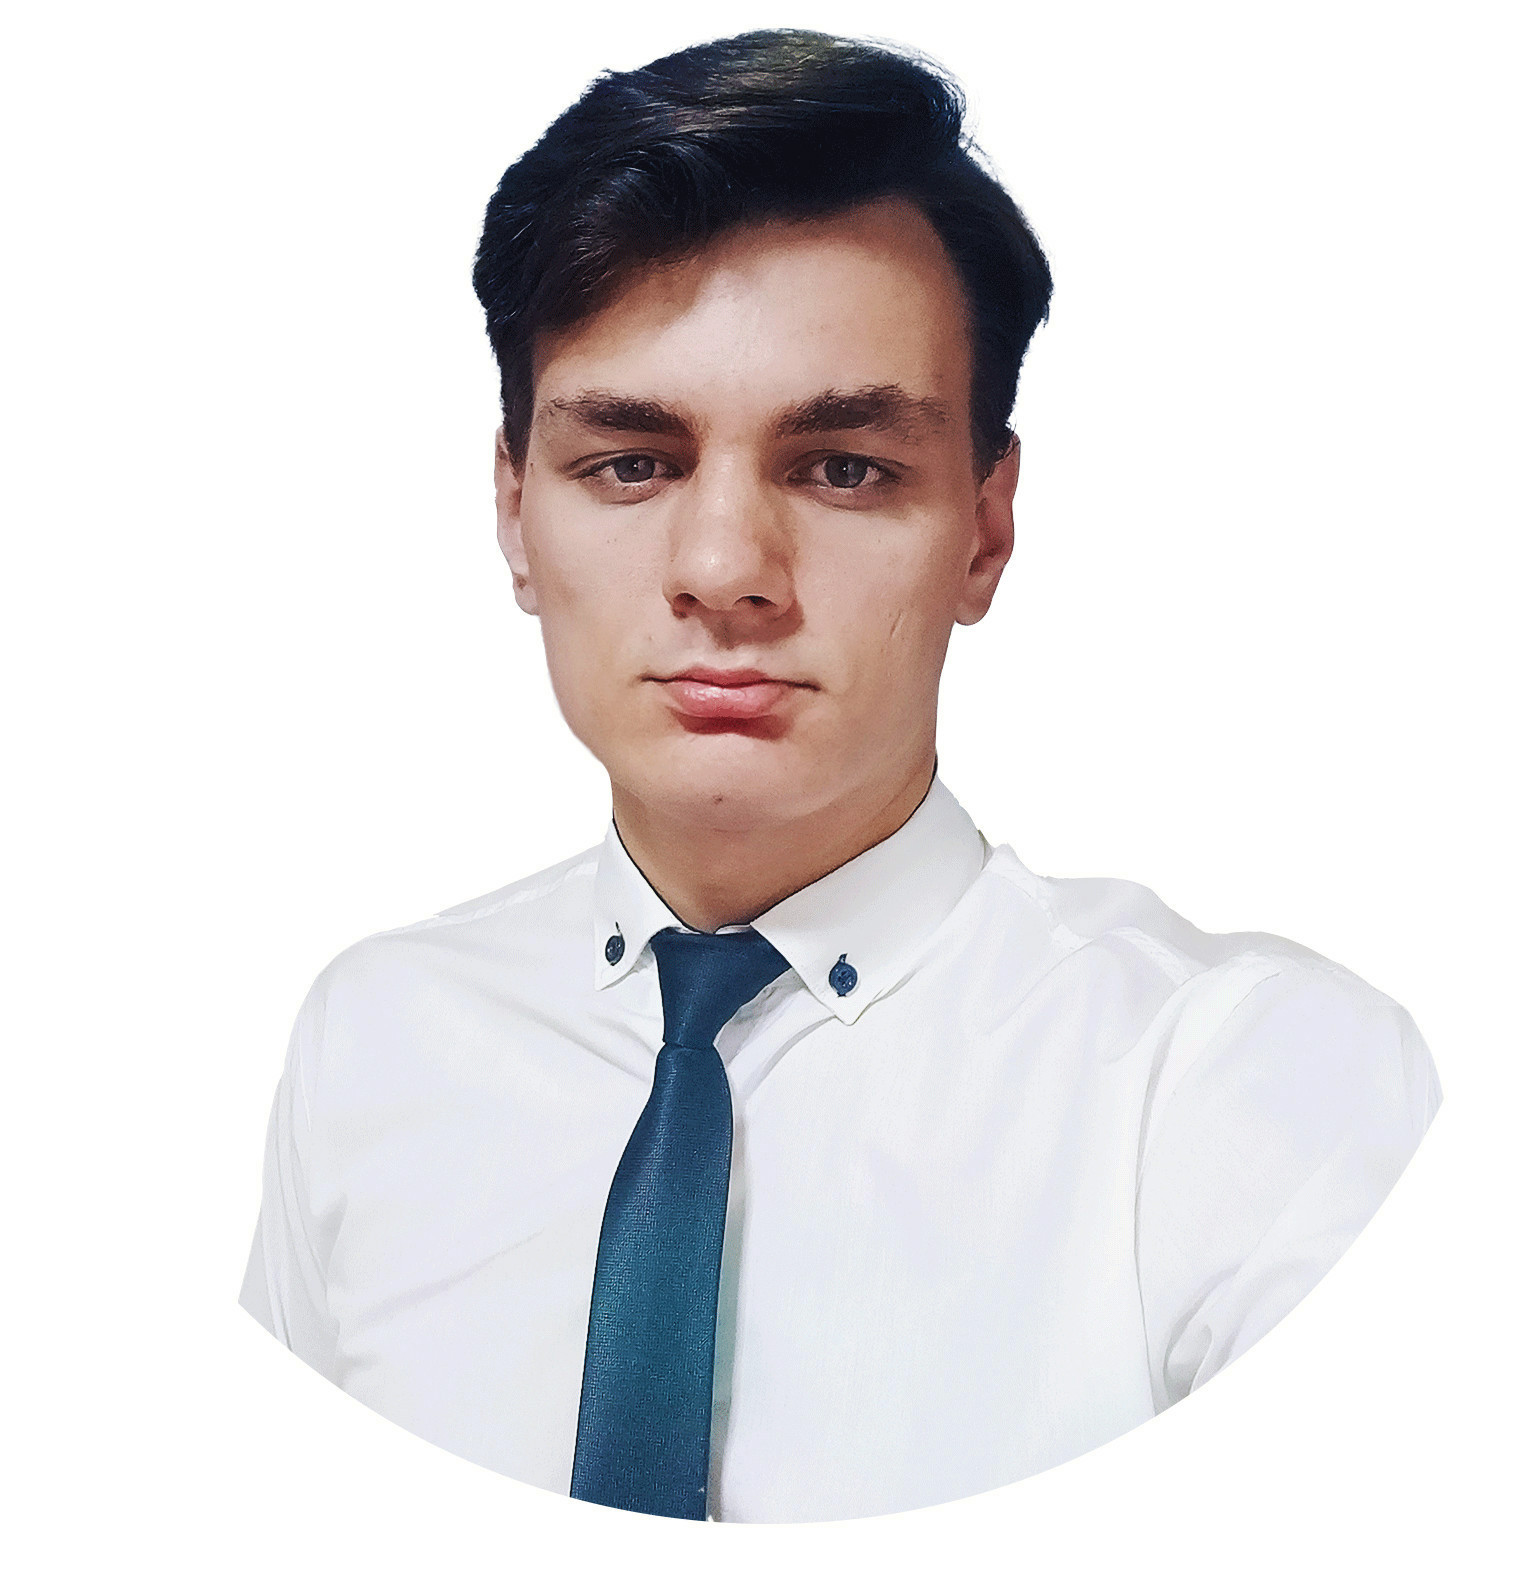
\includegraphics[scale=0.045, center]{foto_cv.jpg}}
\end{minipage}

\vspace{0.5cm}


%----------------------------------------------------------------------------------------
%	EXPERIENCE
%----------------------------------------------------------------------------------------

\cvsect{Esperienza professionale}

\begin{entrylist}
	\entry
	{Settembre 2021 \\ Presente	\\\footnotesize{smart working}}
	{Borsa di Ricerca - Proactive Modules}
	{Università degli Studi di Milano - Bicocca}
	{Attività di ricerca su tecniche di self-repair in Android sfruttando il framework Xposed per rilevare e risolvere a runtime violazioni di policy riguardanti l'utilizzo delle API Android. Sviluppo di tool Eclipse che permeta la generazione di librerie proattive a partire da automi a stati finiti. Lavoro svolto assieme ai professori Daniela Micucci, Leonardo Mariani e Oliviero Riganelli. \\ \texttt{Java}\slashsep\texttt{Eclipse PDE, EMF \& GMF}\slashsep\texttt{Acceleo}\slashsep\texttt{Apache Maven}\slashsep\texttt{Gradle}\slashsep\texttt{Flutter}}
	
	\entry
		{Marzo 2020 \\ Presente \\\footnotesize{smart working}}
		{MindBlooming: una soluzione mobile a supporto della CBT}
		{Università degli Studi di Milano - Bicocca}
		{Continuazione del lavoro iniziato durante lo stage assieme alla prof.ssa Daniela Micucci e al dott. Davide Ginelli in collaborazione col dipartimento di Psicologia UniMiB, aspetto che mi ha permesso di sviluppare molto le mie capacità di lavorare in team, di comunicare e di capire le richieste. \\ \texttt{Java}\slashsep\texttt{Dart}\slashsep\texttt{Flutter}}
	\entry
		{Dicembre 2020 \\ Marzo 2020\\\footnotesize{smart working}}
		{Stage sviluppo cross-platform con Flutter}
		{Università degli Studi di Milano - Bicocca}
		{Sviluppo di una applicazione multi-piattaforma a sostegno della terapia cognitivo comportamentale. Acquisite ottime conoscenze dell'ambiente mobile, soprattutto Android grazie anche al corso di Programmazione di Dispositivi Mobile. Sviluppate anche problem solving, lavoro autonomo, self-learning, adattabilità a soluzioni nuove, lavoro per obiettivi, pianificazione e organizzazione. \\ \texttt{Java}\slashsep\texttt{Dart}\slashsep\texttt{Flutter}}
	\entry
		{3/9/2018  21/9/2018}
		{Elmec SmartCollege}
		{Elmec Informatica S.P.A. - Varese}
		{Corso intensivo di formazione su gestione clienti, web design, sviluppo web e cross-platform, UI e UX Design a diretto contatto con i relativi reparti di Elmec. \\ \texttt{node.js}\slashsep\texttt{Vue.js}\slashsep\texttt{React Native}}
	\entry
		{2016 -- 2018\\\footnotesize{part time}}
		{Grafica Sito web \& Gestione database}
		{Indieversus - Novara}
		{Lavoro svolto durante il triennio liceale comprendente attività di grafica pubblicitaria, UI Design, sviluppo e mantenimento di sito web. Sviluppate anche buona gestione del tempo e capacità di adattamento a contesti lavorativi diversi. \\ \texttt{HTML}\slashsep\texttt{PHP}\slashsep\texttt{JavaScript}\slashsep\texttt{Adobe Photoshop}\slashsep\texttt{Adobe After Effects}}
	\entry
		{2016 -- 2018}
		{Alternanza Scuola Lavoro}
		{ITIS G. Fauser - Novara}
		{Esercitazioni CISCO, esperienze di laboratorio ed incontri informativi su Industria 4.0, Internet of Things e sviluppi futuri dell'informatica. \\ \texttt{C}\slashsep\texttt{C\#}\slashsep\texttt{C++}\slashsep\texttt{Cisco Packet Tracer}}
\end{entrylist}

%----------------------------------------------------------------------------------------
%	EDUCATION
%----------------------------------------------------------------------------------------

\cvsect{Istruzione e formazione}

\begin{entrylist}
	\entry
		{2018 -- 2021}
		{Laurea Triennale}
		{Università Degli Studi di Milano Bicocca}
		{Conseguimento laurea triennale in Informatica con voto 110L/110.}
	\entry
		{2015 -- 2018}
		{Diploma esame di stato - profilo informatico}
		{ITIS G. Fauser - Novara}
		{Voto: cento/centesimi}
	\entry
		{2013 -- 2015}
		{Biennio profilo informatico}
		{ITIS H. Hertz - Roma}
		{Ho svolto i primi due anni di liceo a Roma.}
\end{entrylist}

%----------------------------------------------------------------------------------------
%	ADDITIONAL INFORMATION
%----------------------------------------------------------------------------------------

\begin{minipage}[t]{0.3\textwidth}
	\vspace{-\baselineskip}

	\cvsect{Lingue}
	
	\textbf{Inglese} - C1 certificato CAE\\
	\textbf{Italiano} - Lingua madre\\
	\textbf{Rumeno} - Lingua madre
\end{minipage}
\hfill
\begin{minipage}[t]{0.3\textwidth}
	\vspace{-\baselineskip}
	
	\cvsect{Borse di Studio}
	
	\textbf{TalentAward} - Elmec, 2018 \\
	\textbf{Giuseppe Sironi} - G. Fauser, 2017 \\
	\textbf{Borsa di ricerca} - UniMiB, 2021
\end{minipage}
\hfill
\begin{minipage}[t]{0.3\textwidth}
	\vspace{-\baselineskip}
	
	\cvsect{Patente di guida}
	
	B
\end{minipage}

%----------------------------------------------------------------------------------------

\vskip 0.8em
\cvsect{Dati Personali}

Autorizzo il trattamento dei miei dati personali ai sensi del Decreto Legislativo 30 giugno 2003, n. 196 "Codice in materia di protezione dei dati personali”.

\end{document}
